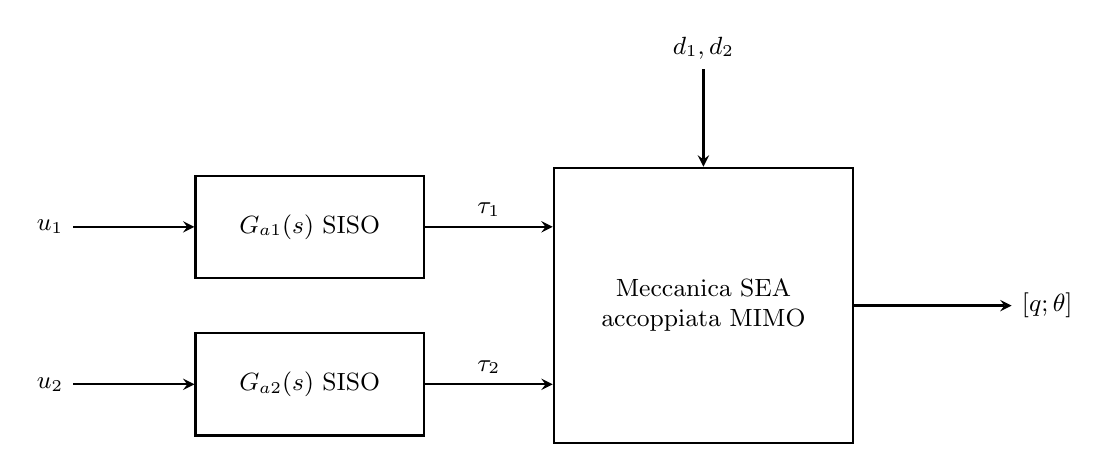
\begin{tikzpicture}[>=stealth,thick,every node/.style={font=\small}]
\node[draw,minimum width=29mm,minimum height=13mm] (a) at (0,1) {$G_{a1}(s)$ SISO};
\node[draw,minimum width=29mm,minimum height=13mm] (b) at (0,-1) {$G_{a2}(s)$ SISO};
\node[draw,align=center,minimum height=35mm,minimum width=38mm] (m) at (5,0) {Meccanica SEA\\accoppiata MIMO};
\draw[->] (-3,1) node[left] {$u_1$} -- (a);\draw[->](-3,-1) node[left] {$u_2$}--(b);
\draw[->](a.east)--(m.west|-a.east) node[midway,above] {$\tau_1$};
\draw[->](b.east)--(m.west|-b.east) node[midway,above] {$\tau_2$};
\draw[->](m.east)--++(2,0) node[right] {$[q;\theta]$};
\draw[->](5,3) node[above] {$d_1,d_2$}--(m.north);
\end{tikzpicture}
